\documentclass[10pt,a4paper]{article}
\usepackage[utf8]{inputenc}

\title{%
  Game Theory: Homework 4 \\
  \large Silvan Hungerbuehler, 11394013}

\usepackage{mathptmx} % "times new roman"
\usepackage{amssymb}
\usepackage{amsmath, amsthm}
\usepackage{amsfonts}
\usepackage{enumitem}
\usepackage{verbatim}
\usepackage{hyperref}
\usepackage{comment}
\usepackage[margin=1in]{geometry}
\usepackage{float}
\usepackage{tikz}
\usetikzlibrary{positioning}

\usepackage[normalem]{ulem}
\date{}
\begin{document}
\maketitle

\section*{Question 1}
\subsection*{a}
\begin{align*}
N=&\{1,2\} \\
A=&\{small,pass,medium,big\} \\
H=&\{A,B\}  &\text{$A$ is the root and $B$ the second player's choice node.}\\
Z=&\{C,D,E\} \\
\underline{i}=&\begin{cases}
A\rightarrow 1 \\
B \rightarrow 2 
\end{cases}&\underline{i}: H\rightarrow N,\text{ maps internal nodes to players} \\
\underline{A}=&\begin{cases}
A\rightarrow\{small,pass\} \\
B\rightarrow\{medium,big\} 
\end{cases} &\underline{A}:H\rightarrow 2^A,\text{ maps internal nodes to available actions} \\
\sigma=& \begin{cases}
\{A,small\}\rightarrow E \\
\{A,pass\}\rightarrow B\\
\{B,medium\}\rightarrow C\\
\{B,big\}\rightarrow D
\end{cases}  &\sigma :H\times A\rightarrow H\cup Z\\
u=&(u_1,u_2)\\
&u_1=\begin{cases}
E\rightarrow 10\\
C\rightarrow 20\\
D\rightarrow 0
\end{cases}\\
&u_2=\begin{cases}
E\rightarrow 0\\
C\rightarrow 20\\
D\rightarrow 30
\end{cases}
\end{align*}
\subsection*{b \& c}
\begin{table}[h]
\centering
\begin{tabular}[l]{|l|l|l|}
\hline
          & $Medium$ & $Big$  \\ \hline
$Small$     & 10, 0   & 10, 0 \\ \hline
$Pass$	& 20,20 & 0, 30 \\ \hline
\end{tabular}
\end{table}
The only pure (subgame-perfect) NE is $(S,B)$. Since $Big$ strictly dominates $Medium$ for Colin, he therefore won't deviate. And Rowena has no incentive to do so either in that strategy profile, because $10>0$.
\subsection*{d} 
Solving the linear equations that represent the players' indifference for $p$ and $q$ yields the mixed NE $[(0,1),(0.5,0.5)]$.
\section*{Question 2}

 \begin{figure}[h]
 	\begin{center}
    \small
    \begin{tikzpicture}[thin,
      level 1/.style={sibling distance=40mm},
      level 2/.style={sibling distance=25mm},
      level 3/.style={sibling distance=15mm},
      every circle node/.style={minimum size=1.5mm,inner sep=0mm}]
      
      \node[circle,draw,label=above:$1$] (root) {}
        child { node {$1,1$}
          edge from parent
            node[left] {$L$}}
        child { node [circle,fill,label=above:$2$] {}
          child { 
            node[circle,fill] (node-A) {}
              child {
                node {$1,1$}
                edge from parent
                  node[left] {$X$}}
              child {
                 node {$8,5$}
                 edge from parent
                   node[right] {$Y$}}
              edge from parent
                node[left] {$A$}}
          child { 
            node[circle,fill] (node-B) {}
              child {
                node {$4,6$}
                edge from parent
                  node[left] {$X$}}
              child {
                 node {$2,1$}
                 edge from parent
                   node[right] {$Y$}}
              edge from parent
                node[right] {$B$}}
           edge from parent
             node[right] {$R$}};
      \draw [dashed] (node-A) -- (node-B) 
         node[midway,above] {$1$};
    \end{tikzpicture}
    \end{center}
    \caption{Extensive-form game $\boldsymbol{G}$}
  \end{figure}
     
\begin{table}[h]
\centering
\caption{Normal-form game $\boldsymbol{G'}$}
\label{my-label}
\begin{tabular}{|l|l|l|}
\hline
      & $A$   & $B$ \\ \hline
$L,X$ & 1, 1 & 1, 1     \\ \hline
$L,Y$ & 1, 1     & 1, 1  \\ \hline
$R,X$ & 1, 1      & 4, 6    \\ \hline
$R,Y$ &  8, 5     & 2, 1    \\ \hline
\end{tabular}
\end{table}

 \begin{figure}[h]
 	\begin{center}
    \small
    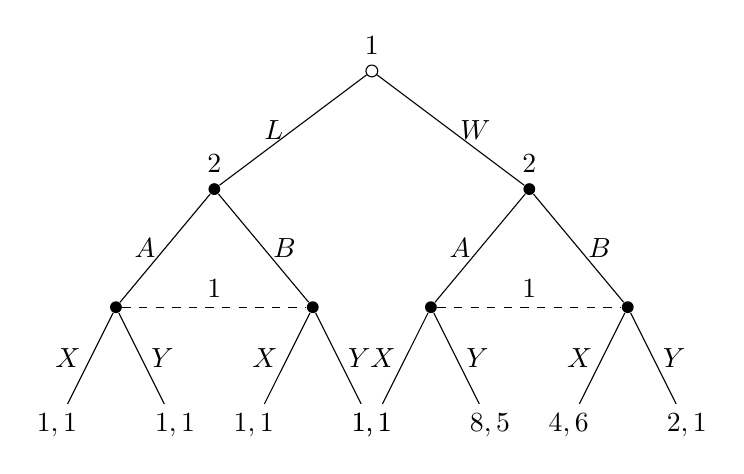
\begin{tikzpicture}[thin,
      level 1/.style={sibling distance=40mm},
      level 2/.style={sibling distance=25mm},
      level 3/.style={sibling distance=15mm},
      every circle node/.style={minimum size=1.5mm,inner sep=0mm}]
      
      \node[circle,draw,label=above:$1$] (root) {}
        child { node [circle,fill,label=above:$2$] {}
          child { 
            node [circle,fill] (node-C) {}
            	child {
            		node {$1,1$}
            		edge from parent
            			node [left] {$X$}}
            	child {
            		node {$1,1$}
            		edge from parent
            			node [right] {$Y$}}
				edge from parent              	
              	node[left] {$A$}}
          child { 
            node [circle,fill] (node-D) {}
            	child {
            		node {$1,1$}
            		edge from parent
            			node [left] {$X$}}
            	child {
            		node {$1,1$}
            		edge from parent
            			node [right] {$Y$}}
            	edge from parent
              	node[right] {$B$}}
          edge from parent
            node[left] {$L$}}
        child { node [circle,fill,label=above:$2$] {}
          child { 
            node[circle,fill] (node-A) {}
              child {
                node {$1,1$}
                edge from parent
                  node[left] {$X$}}
              child {
                 node {$8,5$}
                 edge from parent
                   node[right] {$Y$}}
              edge from parent
                node[left] {$A$}}
          child { 
            node[circle,fill] (node-B) {}
              child {
                node {$4,6$}
                edge from parent
                  node[left] {$X$}}
              child {
                 node {$2,1$}
                 edge from parent
                   node[right] {$Y$}}
              edge from parent
                node[right] {$B$}}
           edge from parent
             node[right] {$W$}};
      \draw [dashed] (node-A) -- (node-B) 
         node[midway,above] {$1$};
      \draw [dashed] (node-C) -- (node-D) 
         node[midway,above] {$1$};
    \end{tikzpicture}
    \end{center}
    \caption{Extensive-form game $\boldsymbol{G''}$}
  \end{figure}
The two extensive-form games are equivalent in the sense that the players can choose the same strategies and all strategy profiles yield the same payoffs.
\end{document}